\capitulo{3}{Conceptos teóricos}

El contenido de este proyecto, mayoritariamente está abarcado dentro de los conceptos de \textit{Minería de Datos} y de \textit{Visión Artificial}. A su vez, se abordarán temas relacionados con el análisis de movimientos y cómo adaptar los resultados obtenidos a lo que se desea interpretar. Para poder poner en práctica todo esto se ha necesitado interiorizar una serie de conceptos clave. Muchos de ellos van a ser expuestos a continuación.

\section{Minería de datos}
A día de hoy cada vez es más frecuente la generación masiva de datos de distintas procedencias y que debido a los avances tecnológicos sean almacenados en grandes bases de datos, haciendo que nos encontremos repletos de los mismos. Esta gran cantidad de datos oculta una fuente de conocimiento inmensa. 

La minería de datos o \textit{Data Mining} es la técnica que estudia métodos y algoritmos por los cuales trata de recopilar nuevas relaciones y patrones entre grandes volúmenes de datos ~\cite{perez2007mineria}. Esto tiene como finalidad poder descubrir y comprender mejor los datos para predecir comportamientos futuros, por ello han surgido nuevas técnicas de aprendizaje automático como puede ser la \textit{Inteligencia Artificial}.


\section{Descubrimiento de Conocimiento en Bases de Datos}

El \emph{Descubrimiento de Conocimiento en Bases de Datos}, en inglés \textit{Knowledge Discovery in Databases} con el acrónimo \emph{KDD}, es una disciplina que tiene como objetivo extraer conocimiento de grandes volúmenes de datos, y que sea usado más adelante para resolver distintos aspectos que al usuario se le pueden plantear ~\cite{fayyad1996kdd}. 

\begin{figure}[H]
    \centering
    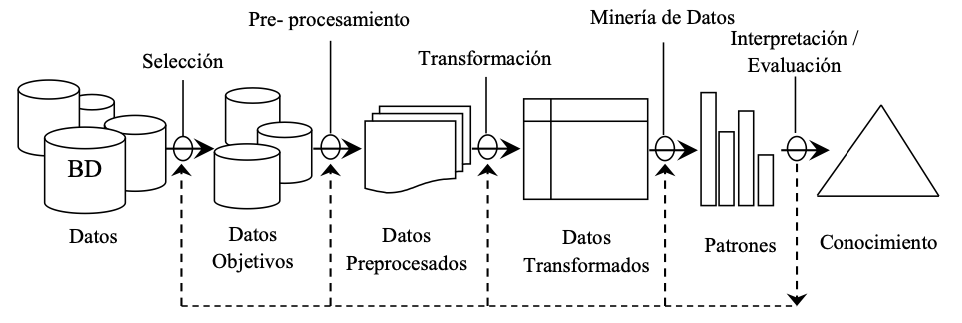
\includegraphics[width=\textwidth]{plantillaLatex-master/img/KDD.png}
    \caption{Proceso KDD.}
    \label{fig:kdd}
\end{figure}

Dentro del \emph{KDD} destacan una una serie de pasos imprescindibles, mostrados en la imagen \ref{fig:kdd}, para llegar al conocimiento buscado, algunos de ellos son los siguientes:
\begin{enumerate}
    \item \textbf{Selección}, este paso busca la creación de un conjunto de datos sobre el que se va a realizar el descubrimiento. En este proyecto los datos de muestra serán una serie de vídeos. 
    \item \textbf{Pre-Procesamiento}, es la etapa que más tiempo consume. En ella se pretende realizar una trasformación de los datos eliminando las características que el usuario considere innecesarias o trasformando los datos según convenga para su estudio. En este proyecto, de cada vídeo analizado se van a extraer los \textit{frames} que lo componen, de cada \textit{frame} se obtendrá el esqueleto del individuo con la pose del cuerpo. Cada pose se guardará dentro de un fichero con las coordenadas de las posiciones. Este fichero será el conjunto de datos procesado.
    \item \textbf{Transformación}, En esta etapa se incluye la extracción de características útiles según el objetivo final. En este proyecto esta será la etapa clave, ya que es en este punto del proceso donde se extraerán las características de cada serie temporal generada y se comparará con otra para poder determinar el objetivo del proyecto. 
    \item \textbf{Interpretación y evaluación}, La evaluación de este proyecto será principalmente visual. El programa informará al usuario sobre los \textit{frames} en los que empieza y termina el vídeo y a través de la aplicación de escritorio se comprobará el resultado. 
\end{enumerate}


\section{Serie temporal}
Una \emph{serie temporal} es una secuencia compuesta por datos obtenidos en diferentes instantes de tiempo y ordenados cronológicamente. Estos datos pueden ser extraídos a partir de una única característica, es lo que se conoce como \emph{series temporales univariantes} o a partir de varias características, \emph{series temporales multivariantes} ~\cite{mauricio2007analisis}.

Una serie temporal compuesta por números naturales tendría la siguiente notación: $X = \{x_1 , x_2, ...\}$ o $\{X_k\}$  $k>=1 $ o $ X = \{X_t : t \in T\}$

Las series temporales que se analizarán en este proyecto serán obtenidas de los distintos \textit{frames}. Cada uno de los \textit{frames} que componen el vídeo será analizado y en caso de obtener exactamente diecisiete puntos en el esqueleto, se almacenarán sus posiciones. Cada una de estas posiciones representar un valor dentro de la serie temporal final. 

Un ejemplo de una buena obtención del esqueleto, y por tanto de las posiciones es la que aparece en la figura \ref{f:esqueletos}.

\section{Visión artificial}

La \emph{visión artificial} intenta emular la capacidad de reconocer escenas presentes en el mundo real y a partir de ello realizar una interpretación para poder actuar en consecuencia ~\cite{marcos2006tecnicas}. De la misma forma que nosotros podemos observar a un paciente y clasificar sus movimientos en función de su agilidad, rapidez o destreza, la visión artificial busca que esa misma clasificación pueda hacerla un ordenador. 

\newpage
\section{OpenCV}

\textit{OpenCV} es una librería libre de visión artificial desarrollada por \textit{Intel}. \textit{OpenCV} significa \textit{Visión Artificial Abierta} o en inglés \textit{Open Computer Vision}. Esta librería es la más popular en el ámbito de la visión artificial y es comúnmente utilizada en campos de investigación sobre detección de objetos, reconocimiento de gestos, detección de movimientos, segmentación y estimación de poses ~\cite{arevalo2004libreria}.

\begin{figure}[H]
    \centering
    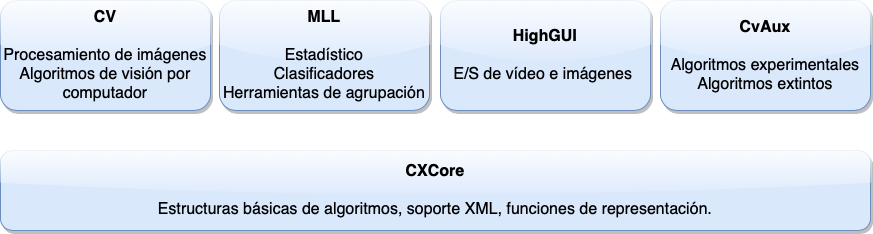
\includegraphics[width=\textwidth]{plantillaLatex-master/img/OpenCV.png}
    \caption{Módulos de la librería \textit{OpenCV}.}
    \label{fig:openCv}
\end{figure}

Se trata de una librería multiplataforma que está dividida en cinco módulos principales, los cuales se pueden observar en la figura \ref{fig:openCv} y son expuestos a continuación:
\begin{enumerate}
    \item \textbf{Módulo CV}, contiene las funciones principales para el procesamiento de imágenes. Además cuenta con numerosos algoritmos de visión por computador.
    \item \textbf{Módulo MLL}, es una biblioteca que incluye múltiples clasificadores estadísticos y proporciona herramientas de clasificación y agrupación para lograr el aprendizaje automático.
    \item \textbf{Módulo HighGUI}, este módulo contiene las funciones básicas para la entrada y salida de vídeos e imágenes. 
    \item \textbf{Módulo CXCore}, este módulo contiene distintas funciones de \textit{OpenCV} y estructuras de datos básicas. 
    \item \textbf{Módulo CvAux}, este módulo contiene tanto áreas extintas como algoritmos experimentales. 
\end{enumerate}

\section{Segmentación}

La \textbf{segmentación} es el proceso por el cual una imagen es fragmentada en distintas regiones, de esta manera se pueden obtener los diferentes objetos de la escena. 

Cabe destacar que en este proyecto es muy importante que el algoritmo elegido para la detección de objetos sepa distinguir a la perfección entre diferentes objetos que puedan aparecer en la escena. De no ser así podría interpretar mal los movimientos del paciente o mezclar las posiciones del esqueleto con las posiciones de otros objetos que reconociese dentro de la imagen. 

\section{Estimación de poses}

La \textbf{estimación de poses} es la clasificación y obtención de las distintas posiciones que toman las articulaciones y partes del cuerpo humanas en vídeos o imágenes ~\cite{garcia2015vision}. 
En esencia, es una forma de detectar un conjunto de \emph{coordenadas} mediante la definición de las articulaciones que componen el cuerpo humano, como pueden ser muñecas, codos, rodillas, etc. 

Las dos técnicas más relevantes de detección de poses humanas son las siguientes ~\cite{wiki:poses}:
\begin{enumerate}
    \item \textbf{Estimación de poses en 2D}, detecta las ubicaciones de las articulaciones del cuerpo humano, y otra serie de puntos clave, como pueden ser los ojos, la nariz o las orejas, en el espacio 2D. De esta manera las posiciones se almacenan como una lista de coordenadas $X$ e $Y$ sobre cada punto clave.
    \item \textbf{Estimación de poses en 3D}, en este caso se representan las articulaciones u otros puntos clave del cuerpo humano a través de tres posiciones. La lista de coordenadas contendrá las posiciones $X$, $Y$, $Z$ de cada punto clave. 
\end{enumerate}


Para la representación de poses humanas se utilizan principalmente tres modelos de estimación que pueden ser observados en la figura \ref{fig:HumanBody} y son expuestos a continuación ~\cite{dang2019deep, s16121966}:
\begin{enumerate}
    \item \textbf{Modelo cinemático}, este modelo también es conocido como el modelo basado en esqueletos e implementa la obtención de coordenadas a partir de los puntos clave del cuerpo humano. Es un modelo intuitivo que es ampliamente utilizado para analizar la relación entre las distintas partes que componen el cuerpo humano.
    \item \textbf{Modelo basado en contornos}, este modelo también conocido como modelo plano y usado para la estimación de poses en 2D, descompone la figura humana en rectángulos y a partir de ellos crea un contorno. De esta forma se obtiene una representación de la forma y apariencia de un individuo.  
    \item \textbf{Modelo basado en volumen}, este modelo se emplea en la estimación de poses en 3D y su representación está basada en aplicar mallas y formas geométricas. A partir de múltiples poses humanas se crea una estimación centrada en el aprendizaje profundo.
\end{enumerate}

\begin{figure}[H]
    \centering
    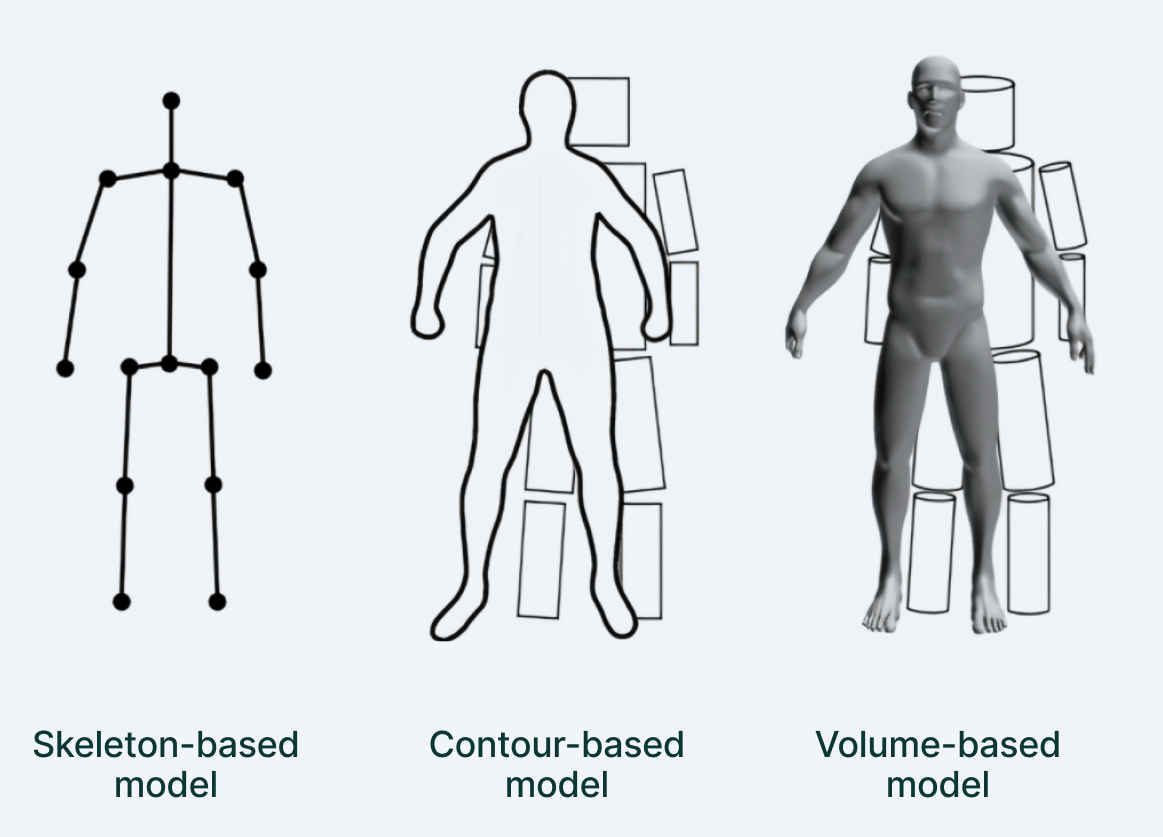
\includegraphics[width=0.9\textwidth]{plantillaLatex-master/img/HumanBodyModels.png}
    \caption{Modelos para la detección de poses humanas.}
    \label{fig:HumanBody}
\end{figure}

Este proyecto se abarcará utilizando una estimación de poses basada en esqueletos. Por ello es importante conocer como se ha implementado la estructura básica del modelo. En las figuras \ref{f:esqueletos_1} y \ref{f:esqueletos_2} se muestra la creación de esqueletos y la numeración de los puntos clave que se han considerado. 


\begin{figure}
 \centering
  \subfloat[\textit{Esqueleto sobre un fondo negro}]{
   \label{f:esqueletos_1}
    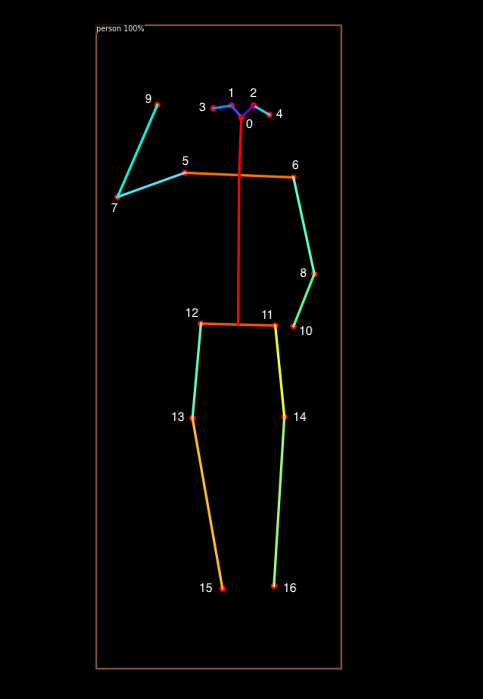
\includegraphics[width=0.48\textwidth]{PosesBlackBackground.png}}
  \subfloat[\textit{Esqueleto sobre el fondo real}]{
   \label{f:esqueletos_2}
    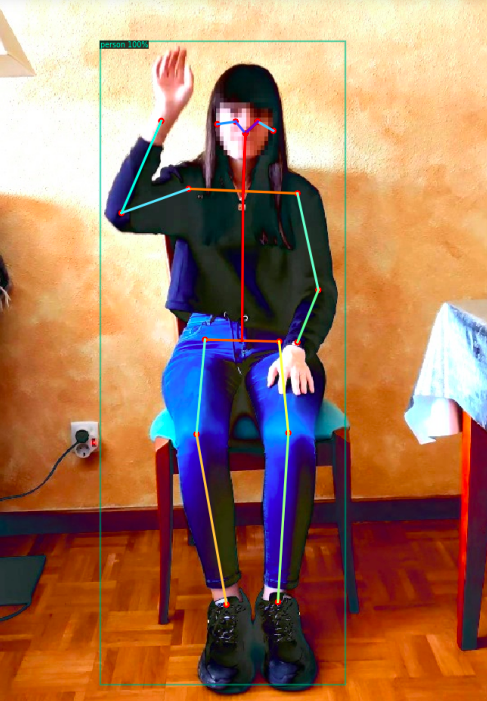
\includegraphics[width=0.47\textwidth]{PosesBackground.png}}
 \caption{Extracción de esqueletos.}
 \label{f:esqueletos}
\end{figure}


\section{Redes Neuronales convolucionales} \label{cap:convolucional}

Las \textbf{redes neuronales convolucionales} con el acrónimo en inglés \textit{CNN}, son un tipo de Red Neuronal Artificial que proporciona la capacidad de \textit{"ver"} al ordenador. Esto lo realiza procesando cada una de sus capas de forma similar a como lo realiza el \textit{cortex} visual del ojo humano. Por esta razón son ampliamente usadas en tareas de visión artificial o clasificación y segmentación de imágenes ~\cite{CRUZ2021103530}.

Estas redes están estructuradas alternativamente en capas de convolución y capas de reducción. Las capas de convolución son las encargadas de extraer patrones dentro de los datos de entrada, mientras que las capas de agrupación se encargan de reducir la resolución de los datos de entrada. A su vez, cada una de estas capas está compuesta por un cierto número de mapas de características. En la figura \ref{f:cnn} se puede observar la estructura de estas redes.

\begin{figure}[H]
 \centering
    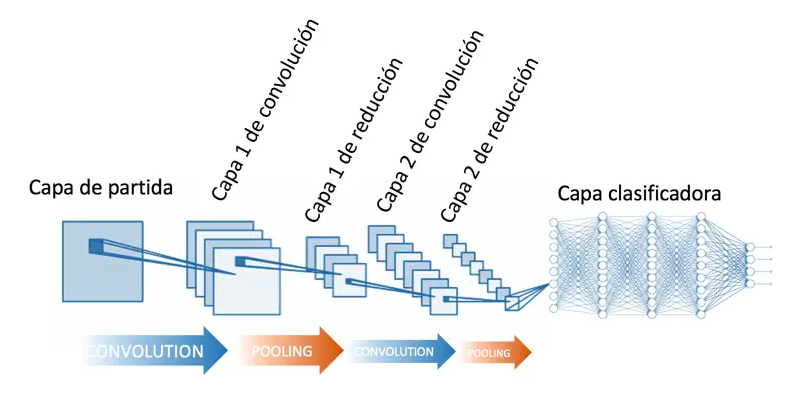
\includegraphics[width=0.72\textwidth]{plantillaLatex-master/img/cnn.png}
    \caption{Arquitectura de una Red Neuronal Convolucional.}
    \label{f:cnn}
\end{figure}

Los principales componentes de la arquitectura \textit{CNN} son ~\cite{bonilla2020redes}:
\begin{enumerate}
    \item Capa convolucional.
    \item Capa de agrupación.
    \item Capa de unidades lineales rectificadas \textit{ReLu}.
    \item Capa completamente conectada.
    \item Capa de pérdida.
\end{enumerate}


\subsection{Capa convolucional (Convolutional layer)}

Es la capa principal en las redes neuronales y pueden usarse desde una a varias capas de este tipo. Las \textbf{capas convolucionales} reciben como parámetros un conjunto de filtros que serán aplicados sobre la imagen de entrada generando un mapa de características o mapa de activación bidimensional para cada filtro. Una vez obtenidos los diferentes mapas de características para todos los filtros se genera como salida la capa convolucional.  

\textbf{Mapa de características}:
\[h^{k}_i_,_j = tanh((w^{k}x)_i_,_j + b_k)\]

Donde $w^{k}$ es el peso, $b_k$ es el sesgo, $x$ es el valor del píxel específico y $tanh$ especifica la no linealidad de los datos. Los subíndices \emph{i}, \emph{j} hacen referencia a las distintas entradas en la matriz que representa el mapa de características.

\subsection{Capa de agrupación (Pooling layer)}
Las capas de agrupación o reducción son comúnmente colocadas entre las distintas capas de convolución y es que su función es la de tomar los mapas de características generados en la capa de convolución previa y agruparlos en una única imagen. 

Para poder reducir el número de parámetros que componen la red neuronal se utiliza la operación de \textit{pooling}, actualmente la agrupación mediante \textit{max-pooling},$f = max$, ha demostrado dar los mejores resultados, es por esa razón que es la más usada pero no hay ningún impedimento en usar cualquier otra función. 

\begin{figure}
 \centering
    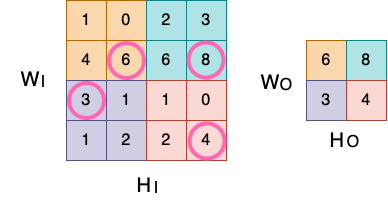
\includegraphics[width=0.72\textwidth]{plantillaLatex-master/img/pooling2.png}
    \caption{Operación de \textit{max-pooling}, filtro 2×2 y S=2.}
    \label{f:pool_2}
\end{figure}


Para un volumen $I=(W_I;H_I;D)$ donde $I={I_1...I_D}$, la operación de agrupación producirá un volumen de salida $O=(W_O;H_O;D)$ donde $O={O_1...O_D}$, deslizando un filtro  $2k$×$2k$, que representa el muestreo de respuesta de la función $f$ que se aplica para disminuir la cantidad de parámetros. En la figura \ref{f:pool_2} se puede observar el resultado de la operación de agrupación con $f=max$ Y $S=2$ . El parámetro $S$ indicará los saltos que irá realizando el filtro, es decir, el número de píxeles que se deberá de desplazar el filtro antes de realizar nuevamente la operación. Finalmente esta operación generarán un volumen resultante con unas dimensiones $W_O= W/2, H_O=H/2, D$ y reduciendo en un 75\% la cantidad e parámetros de entrada para poder seguir con el entrenamiento. 

\subsection{Capa de unidades lineales rectificadas ReLu (Rectified Linear Units Layer)}

La capa \textit{Rectified Linear Units} o \emph{ReLu} tiene como principal funcionalidad aumentar las propiedades de no linealidad de la función de activación, y no necesitan parámetros, si no que utilizan una función fijada. La función más utilizada es $f(x) = max(0,x)$ aunque se pueden usar otras como $f(x) = tanh(x)$ que permite entrenar con una mayor rapidez o $f(x) = |tanh(x)|$.

\subsection{Capa completamente conectada (Full connected layer)}

Esta capa, como su propio nombre indica, es una capa con una arquitectura completamente conectada por lo que no utiliza propiedades de conectividad local. El único parámetro que se puede configurar de este tipo de capas, es el número de neuronas que componen la capa, y es que cada neuronas de esta capa se encuentran conectadas a todos los mapas de características de la capa anterior. 

Como parámetro de salida genera un único vector $1$×$1$×$K$ que contiene las activaciones calculadas. Al generar una sola dimensión como salida, esta capa indica que tras ella no podrá haber más capas convolucionales. El parámetro $K$ que se obtiene en la salida se usará en la siguiente capa con una función probabilística para realizar la clasificación.  

\subsection{Capa de pérdida (Loss layer)}
Esta capa es la que se encarga de la comparación entre las predicciones obtenidas y los valores reales de la imagen. Para esta operación se pueden usar una función de pérdida \textit{softmax} o una función de pérdida euclídea.  

\textbf{Función de pérdida \textit{softmax}}
\begin{equation}
\sigma(Z)_j=\frac{e^{z_j}}{\sum_{k=1}^{K}e^{z_k}}
\end{equation}

\begin{equation}
z_j=\sum_{k=0}^{d}W_{ik}x_k
\end{equation}
donde:
\begin{enumerate}
    \item $z_j$, es el vector de probabilidad.
    \item $j$, es la \textit{i−ésima} neurona de la capa de pérdida.
    \item $K$, es el número total de neuronas de la capa de pérdida.
    \item $W_k_i$, son los pesos.
    \item $x_i$, son los valores de entrada de la capa de pérdida.
    \item $σ(z)_j$, es la activación de las $K$ neuronas de la capa de pérdida.
\end{enumerate}

\textbf{Función de pérdida \textit{euclídea}}
\begin{equation}
E=\frac{1}{2K}\sum_{i=1}^{K}||\hat{y}_i-y_i||^{2}_2
\end{equation}
donde:
\begin{enumerate}
    \item $K$, es el número total de neuronas de la capa de pérdida.
    \item $\hat{y}_i$, son las predicciones de las imágenes.
    \item $y_i$, son los valores reales de las imágenes.
\end{enumerate}


\section{Dynamic Time Warping} \label{cap:DTW}
\subsection{Introducción}
\textbf{Dynamic Time Warping} (DTW) es un algoritmo creado para la alineación de secuencias temporales no lineales tratando de encontrar una ruta de alineación óptima ~\cite{muller2007dynamic}. Es ampliamente utilizado en el campo del reconocimiento por voz, la detección y clasificación de movimientos y gestos humanos y el reconocimiento de formas y firmas. Es utilizado en estos ámbitos porque lo que \emph{DTW} consigue es una alineación de puntos de tiempo muy similares en diferentes instantes de tiempo.

En la figura \ref{fig:dtw1} se puede observar como el algoritmo \emph{DTW} realiza una alineación de puntos entre dos secuencias.

\begin{figure}[H]
    \centering
    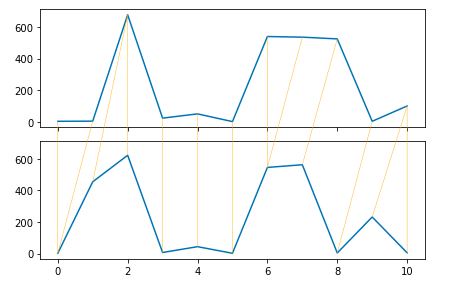
\includegraphics[width=0.7\textwidth]{plantillaLatex-master/img/DTW_alignment.jpg}
    \caption{Alineación \textbf{DTW} entre dos secuencias.}
    \label{fig:dtw1}
\end{figure}

Dadas dos secuencias $X:=(x_1, x_2 ... x_N)$ e $Y:=(y_1, y_2 ... y_M)$ en las que $M \in$ $N$, el objetivo del algoritmo \emph{DTW}será encontrar una alineación óptima entre ambas secuencias. En la figura \ref{fig:dtw2} se muestra una posible alineación de secuencias señalizada por las flechas moradas bidireccionales.


\begin{figure}[H]
    \centering
    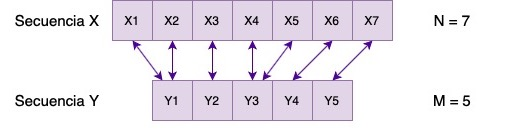
\includegraphics[width=\textwidth]{plantillaLatex-master/img/DTW_sequences.jpg}
    \caption{Alineación teórica \textbf{DTW} entre dos secuencias.}
    \label{fig:dtw2}
\end{figure}

Cada una de las flechas indica una relación entre los valores $x_n$ e $y_m$ para $n \in $  $[1:N]$ y $m \in$ $[1:M]$ 


\subsection{Camino de deformación DTW}
Un camino de deformación determina la alineación entre dos secuencias. Esta alineación es creada a partir de la matriz de costes que crea el algoritmo de \emph{DTW}. Este camino o ruta de deformación cuenta con una longitud $L \in$ $N$ creando una secuencia $P = (p_1, p_2 ... p_L) $ que cumpla las siguientes condiciones ~\cite{bishop2006pattern}: 
\begin{enumerate}
    \item \textbf{}{Condición de límite}, esta restricción especifica que tanto los puntos de inicio como de fin de ambas señales, son emparejados entre ellos.
    \begin{equation}
        p_1 = (1,1) \quad \& \quad p_L = (N,M)
    \end{equation}
    \item \textbf{Condición de monotonicidad}, esta restricción hace que se cumpla con un orden temporal en la asignación de los elementos.
    \begin{equation}
        n_1 <= n_2 <= ... <= n_L \quad \& \quad m_1 <= m_2 <= ... <= m_L
    \end{equation}
    \item \textbf{Condición de continuidad}, restringe los saltos en el tiempo y ciñe los cambios a puntos contiguos.
    \begin{equation}
        l \in [1:L]  n_l - n_l_-_1 <= 1 \quad \& \quad m_l - m_l_-_1 <= 1
    \end{equation}
    o lo que es lo mismo:
    \begin{equation}
        p_l - p_l_-_1  \in \sum := \{(1,0),(0,1),(1,1)\}
    \end{equation}
\end{enumerate}

También existen otras restricciones menos frecuentes 
\begin{enumerate}
    \item \textbf{Condición de ventana deformada}, esta restricción permite crear una selección de puntos a partir de un valor por defecto, escogiendo solo aquellos que cumplan dicha restricción. 
    \begin{equation}
        l \in [1:L] \quad \& \quad |n_l - m_l | <= (\sigma)
    \end{equation}
    \item \textbf{Condición de la pendiente}, esta restricción permite crear una ruta de deformación a partir de una limitación en cuanto a la pendiente. De esta manera se podrán evitar los movimientos bruscos en un determinado sentido.
\end{enumerate}


\subsection{Matriz de costes locales}

Para poder localizar una ruta de deformación óptima es necesaria la presencia de una matriz de distancias o matriz de costes \textit{C} representada en la figura \ref{fig:dtw3} ~\cite{zhang2020dynamic}. Teniendo en cuenta las secuencias $X:=(x_1, x_2 ... x_N)$ e $Y:=(y_1, y_2 ... y_M)$ si c(x,y) son similares, el valor que proporcionará la matriz será bajo, mientras que si son muy dispares, ese mismo valor c(x,y) será elevado. Evaluando cada una de las combinaciones de la secuencia $X$ con la secuencia $Y$ se consigue la \textbf{matriz de costes locales} $C \in R _N$x$M $ con $n \in [1:N]$ y $m \in [1:M]$ definida como:
\begin{equation}
C(n,m):=c(x_n,y_m)   
\end{equation}

\begin{figure}
    \centering
    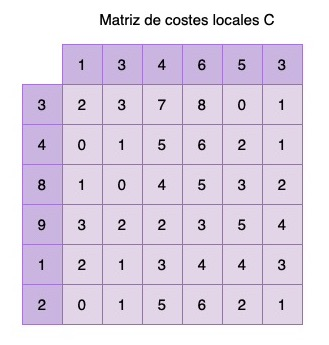
\includegraphics[width=0.5\textwidth]{plantillaLatex-master/img/DTW_matrix_C.jpg}
    \caption{Matriz de coses locales.}
    \label{fig:dtw3}
\end{figure}

Para calcular esta matriz hace falta especificar una métrica de cálculo la distancia entre dos puntos \cite{jain2017optimal}. En los ejemplos se han realizado las comparaciones con la distancia euclidiana.

\subsection{Matriz de costes acumulados}

Esta nueva matriz $D \in R _N$x$M $ con $n \in [1:N]$ y $m \in [1:M]$ se define a partir de las siguientes condiciones:
\begin{enumerate}
    \item La primera fila de D está inicializada como:
    \begin{equation}
        D(1,m):=C(1,m)  
    \end{equation}
    \[m \in [1:M]\]
    \item La primera columna de D está inicializada como:
    \begin{equation}
        D(n,1):=\sum_{k=1}^{n}C(k,1)  
    \end{equation}
    \[n \in [1:N]\]
    \item El resto de los valores se definen recursivamente a partir de la matriz de costes locales:
    \begin{equation}
        D(n,m)=C(n,m)+min\left\{(D  n−1,m−1),D(n−1,m),D(n,m−1)\right\}
        \end{equation}
        \[n \in [2:N]\] 
        \[m \in [2:M]\]
    
\end{enumerate}

\begin{figure}
    \centering
    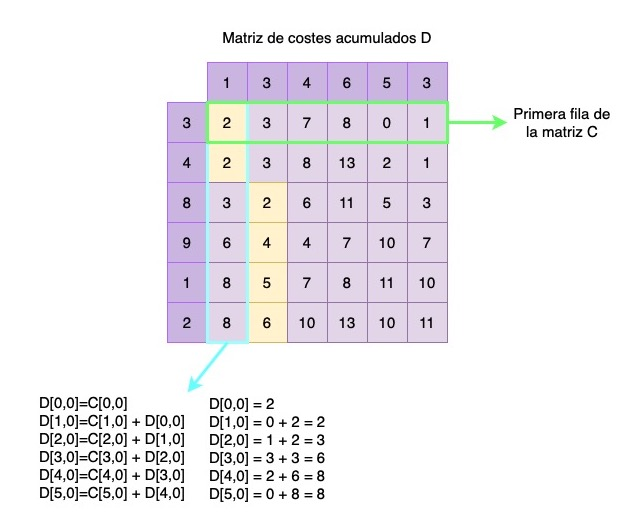
\includegraphics[width=0.9\textwidth]{plantillaLatex-master/img/DTW_matrix_D_2.jpg}
    \caption{Matriz de coses acumulados.}
    \label{fig:dtw4}
\end{figure}

En la figura \ref{fig:dtw4} se puede apreciar como a partir de la matriz de costes locales se ha obtenido la matriz de coses acumulados. 

\newpage
\subsection{Ruta de deformación}
Dentro de la matriz de costes acumulados se podrán realizar los siguientes saltos para la elección del camino óptimo:
\begin{enumerate}
    \item \textbf{Movimientos horizontales}, C(n,m) $\Rightarrow$ C(n,m+1) \\
    \item \textbf{Movimientos verticales}, C(n,m) $\Rightarrow$ C(n+1,m) \\
    \item \textbf{Movimientos diagonales}, C(n,m) $\Rightarrow$ C(n+1,m+1)
\end{enumerate}

Si se tiene una secuencia a localizar, $X:=(x_1, x_2 ... x_N)$ y una secuencia de mayor tamaño $Y:=(y_1, y_2 ... y_M)$ en la que buscar la primera secuencia. Una ruta de deformación será el camino que especifique las alienaciones entre la secuencia a alinear y los valores más similares a ella dentro de la segunda secuencia, que pueden compartir las misma longitud o no. Esta ruta de deformación estará compuesta por tuplas en las que el primer elemento indique la posición de la secuencia de referencia, o la secuencia que se desea alinear y el segundo elemento indicará la posición de la alineación de dicho elemento dentro de la segunda secuencia. 


\section{Búsqueda de secuencias}
Dadas dos secuencias $ X := ( x_{1}, x_{2}, x_{3} ... x_{N}) $ e $ Y := ( y_{1}, y_{2}, y_{3} ... y_{M}) $ con $ N < M $ el objetivo es localizar una secuencia lo más semejante posible a la secuencia $X$ denominada patrón de referencia, dentro de una secuencia de mayor tamaño $Y$, y que asimismo, informe sobre en que punto se ha localizado dicha secuencia. 
El objetivo será trabajar con secuencias multidimensionales pero anteriormente se realizarán múltiples ejemplos con secuencias unidimensionales hasta conseguir un óptimo funcionamiento. 

En la figura \ref{fig:dtw5} se muestra una alineación indicada por las flechas bidireccionales azules, entre el patrón de referencia $X$ de longitud $N=4$ y una secuencia muy parecida al mismo ubicada en una serie temporal $Y$ de mayor tamaño $M=10$

\begin{figure}
    \centering
    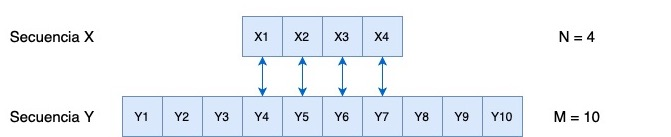
\includegraphics[width=\textwidth]{plantillaLatex-master/img/Subsequence.jpg}
    \caption{Alineación teórica de secuencias.}
    \label{fig:dtw5}
\end{figure}

Cada una de las flechas bidireccionales azules crea una correspondencia entre dos elementos $x_n$ e $y_m$ para $n \in [1:N]$ y $m \in [1:M] $.


\subsection{Formalización del problema}
Para modelar matemáticamente nuestro problema de búsqueda de secuencias, consideramos que la longitud de $M$ es mucho mayor que la de $N$ y que existe una matriz de costes locales $C$ dada por $C(n,m)=c(x_n,y_m)$ para $n \in [1:N] $ y $m \in [1:M] $ y una matriz de costes acumulados $D$ definida según las restricciones comentadas anteriormente con un tamaño igual al de la matriz de costes locales $C$. Finalmente para denotar  una subsecuencia de $Y$ se utilizarán los índices $a,b \in [1:M]$ con $a<=b$ y la notación:
\begin{equation}
    Y(a:b):=(y_a, y_{a+1},... y_b)
\end{equation}
